\documentclass{article}
\usepackage[utf8]{inputenc}
\usepackage{amsmath, amssymb, bm}
\usepackage{gensymb}
\usepackage{graphicx}

\begin{document}
	\textbf{Trig Inequality 1:} For all angles $\theta > 0$,
	$$\sin{(\theta)} < \theta$$
	\textbf{Proof:}
	Let $\theta > 0$ be an arbitrary real angle. \\\\
	Case 1: Suppose $\theta \geq \frac{\pi}{2}$. Since the range of sine is $[-1, 1]$, then
	$$\sin{(\theta)} \leq 1$$
	Since $\frac{\pi}{2} \approx 1.571 > 1$, then
	\begin{align*}
		\sin{(\theta)} < \frac{\pi}{2} \leq \theta
	\end{align*}
	which is what we wanted to show. \\\\
	Case 2: Suppose $0 < \theta < \frac{\pi}{2}$. Then the terminal side of the angle $\theta$ lies in Quadrant 1 and can be represented by Figure 1 below.
	\begin{figure}[h!]
		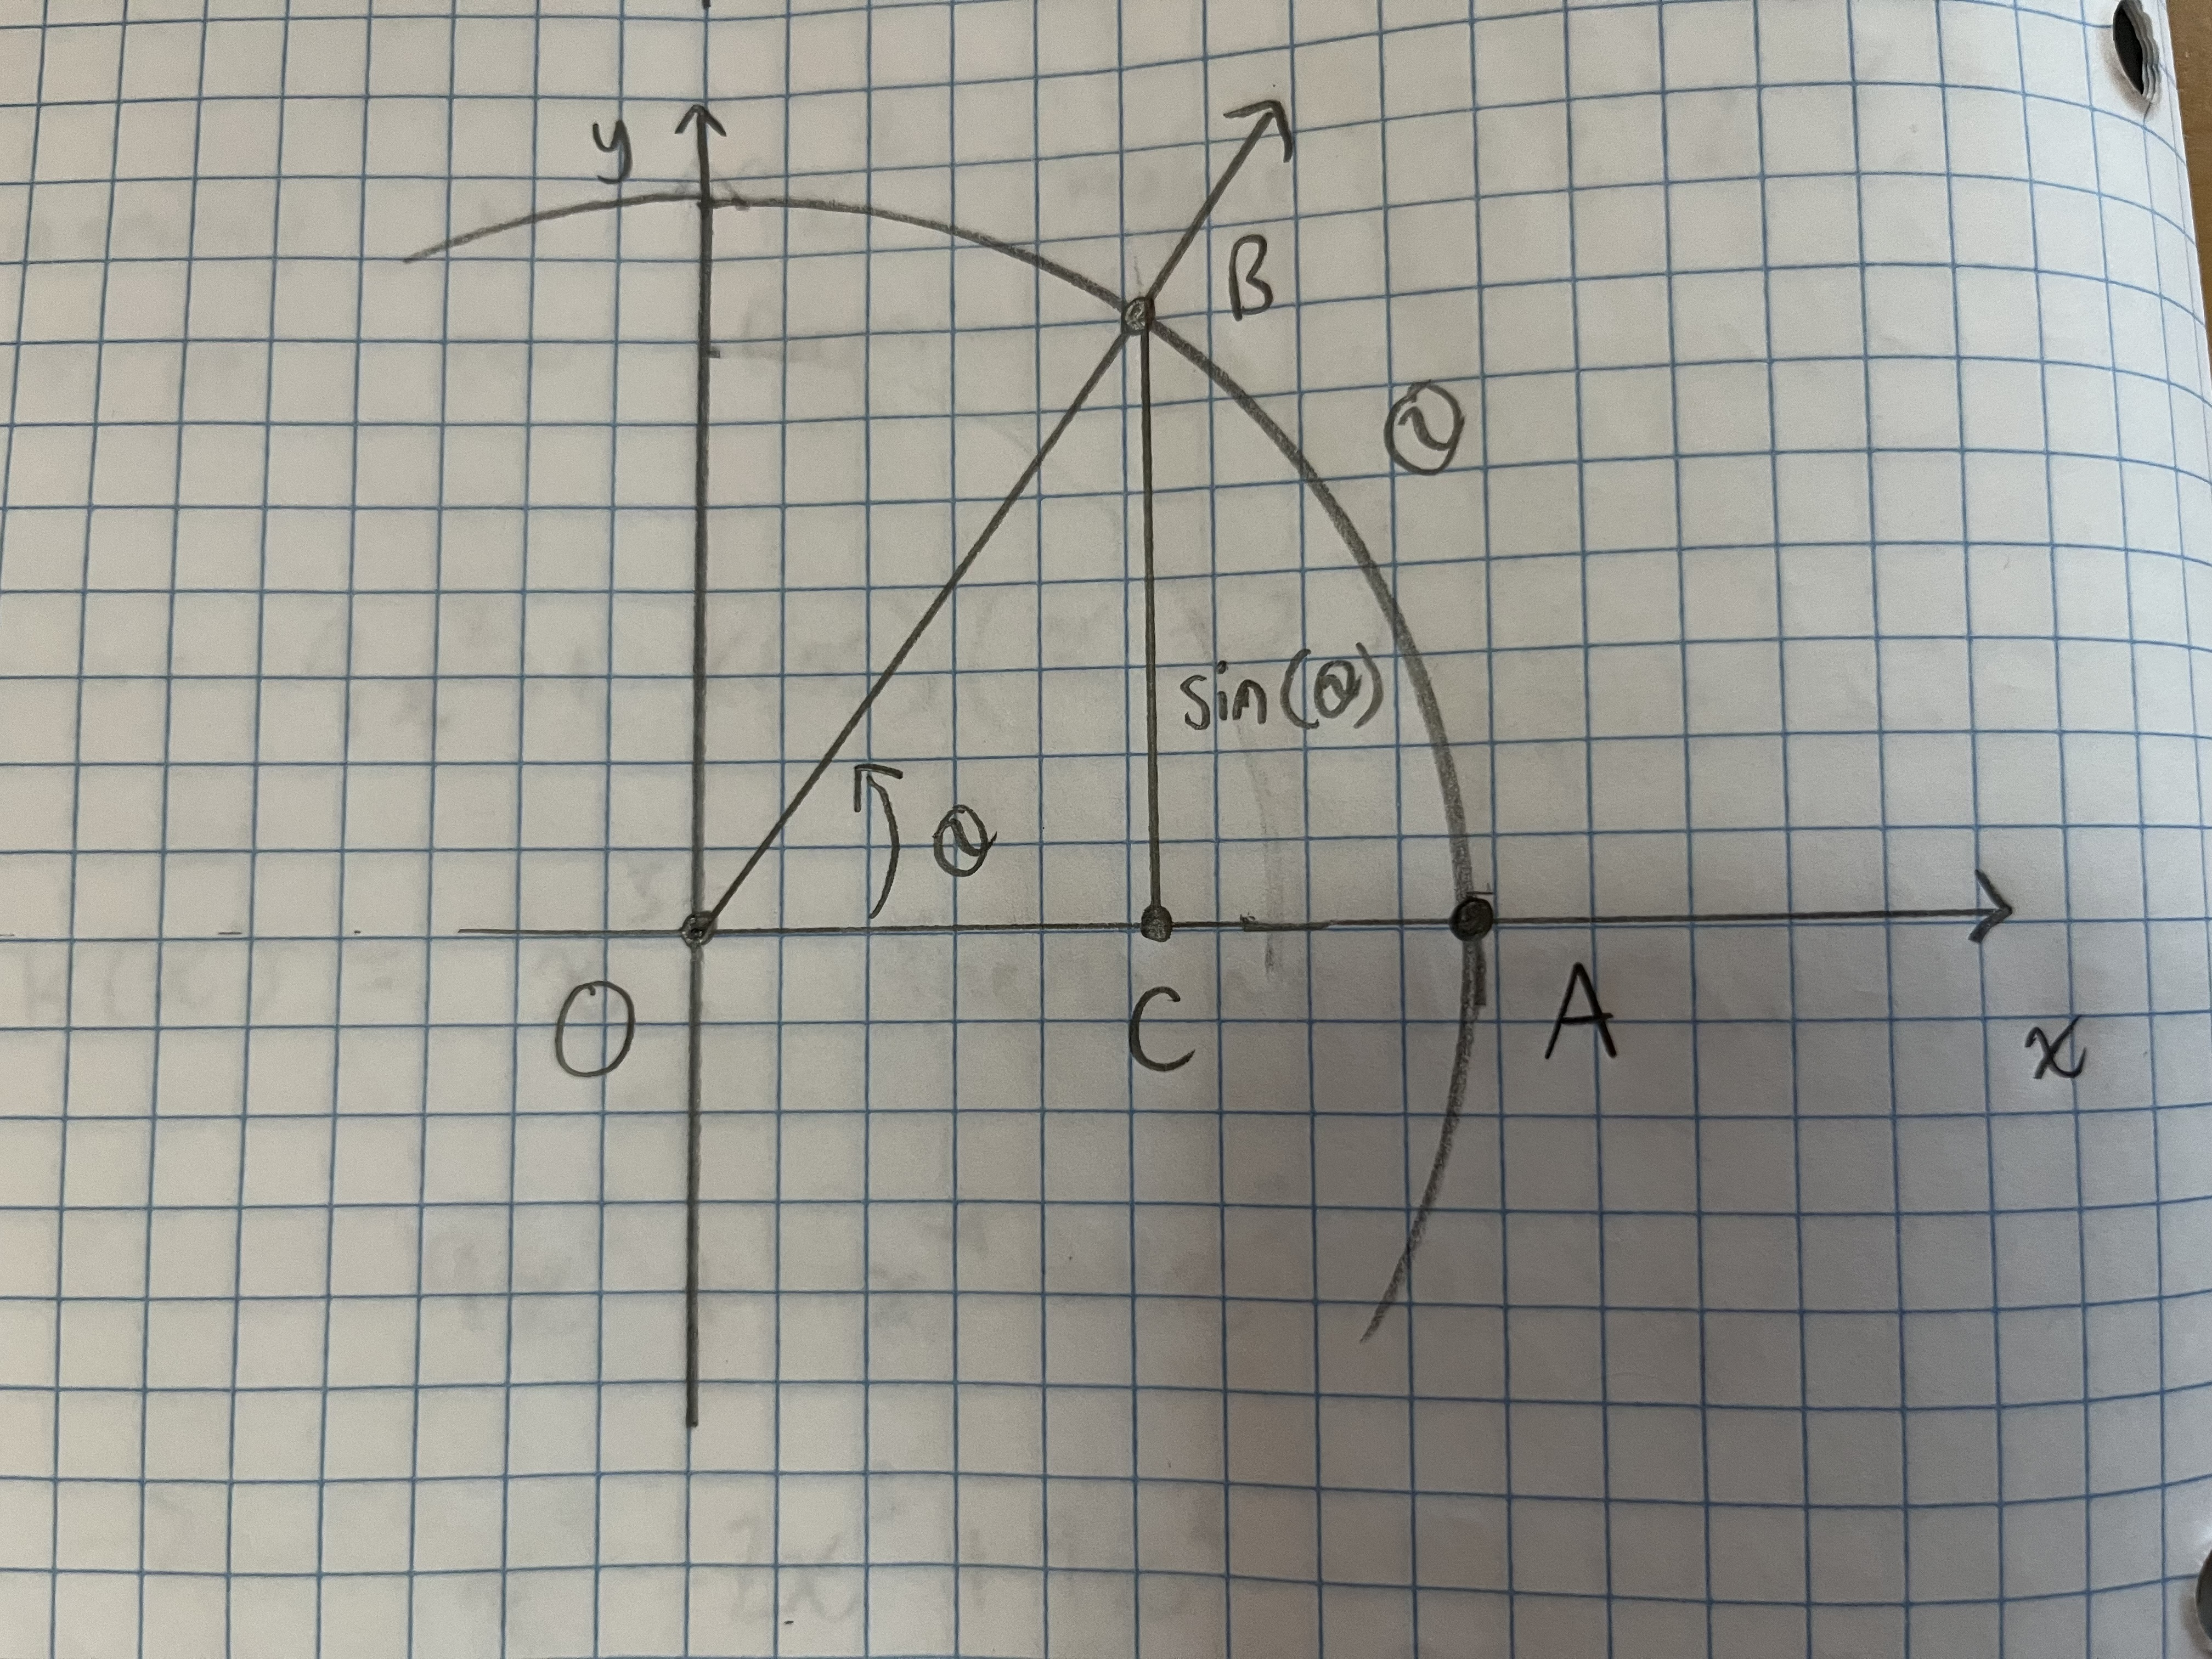
\includegraphics[width=\linewidth]{Trig_Figure.JPG}
		\caption{Angle lies in Q1}
	\end{figure} \\
	By definition, $\sin{(\theta)} = |BC|$. By the definition of radian measure, the length of arc $AB = \theta$. From looking at the figure, it is geometrically intuitive \footnote{This is all we can say without having access to a more precise definition of arc length.} that the arc $AB$ is a longer length than the line segment $BC$.
	
	Therefore
	\begin{align*}
		|BC| &< \text{arc } AB \\
		\sin{(\theta)} &< \theta
	\end{align*}
	
	The inequality holds in both cases, so it is true for all $\theta > 0$.
\end{document}